\documentclass[10.5pt]{article}

\usepackage{amsmath,amssymb}
\usepackage{bm}
\usepackage{geometry}
\usepackage{ctex}
\usepackage{setspace}
\usepackage{graphicx}
\usepackage{float}
\geometry{a4paper,margin=2cm}

%========================
% 排版设置
%========================
\setstretch{1.2}
\setlength{\parskip}{4pt}
\setlength{\parindent}{2em}

\setlength{\abovedisplayskip}{5pt}
\setlength{\belowdisplayskip}{5pt}
\setlength{\abovedisplayshortskip}{3pt}
\setlength{\belowdisplayshortskip}{3pt}

% 标题编号
\setcounter{secnumdepth}{3}

\title{\textbf{Kondo effect：理论模型与低温输运特征}}
\author{Super}
\date{}

\begin{document}

\maketitle

\section{Kondo效应定义}

Kondo效应是一种由局域磁矩(local magnetic moment)与导电电子之间反铁磁交换耦合产生的量子多体效应。在低温条件下，导电电子通过自旋翻转散射逐渐屏蔽局域磁矩，并形成Kondo单态(Kondo singlet)，从而增强电子散射，使材料电阻随温度降低出现反常升高。

对于传统金属，低温电阻通常由于电子-声子散射减弱而降低。而在Kondo体系中，磁性散射贡献可表示为：
\begin{equation}
\rho(T)=\rho_0-A\ln T ,
\end{equation}
其中$\rho_0$为残余电阻，$A$为Kondo散射系数。低温区域的$\rho\sim-\ln T$关系是Kondo效应最重要的输运特征。
\begin{figure}[H]
    \centering
    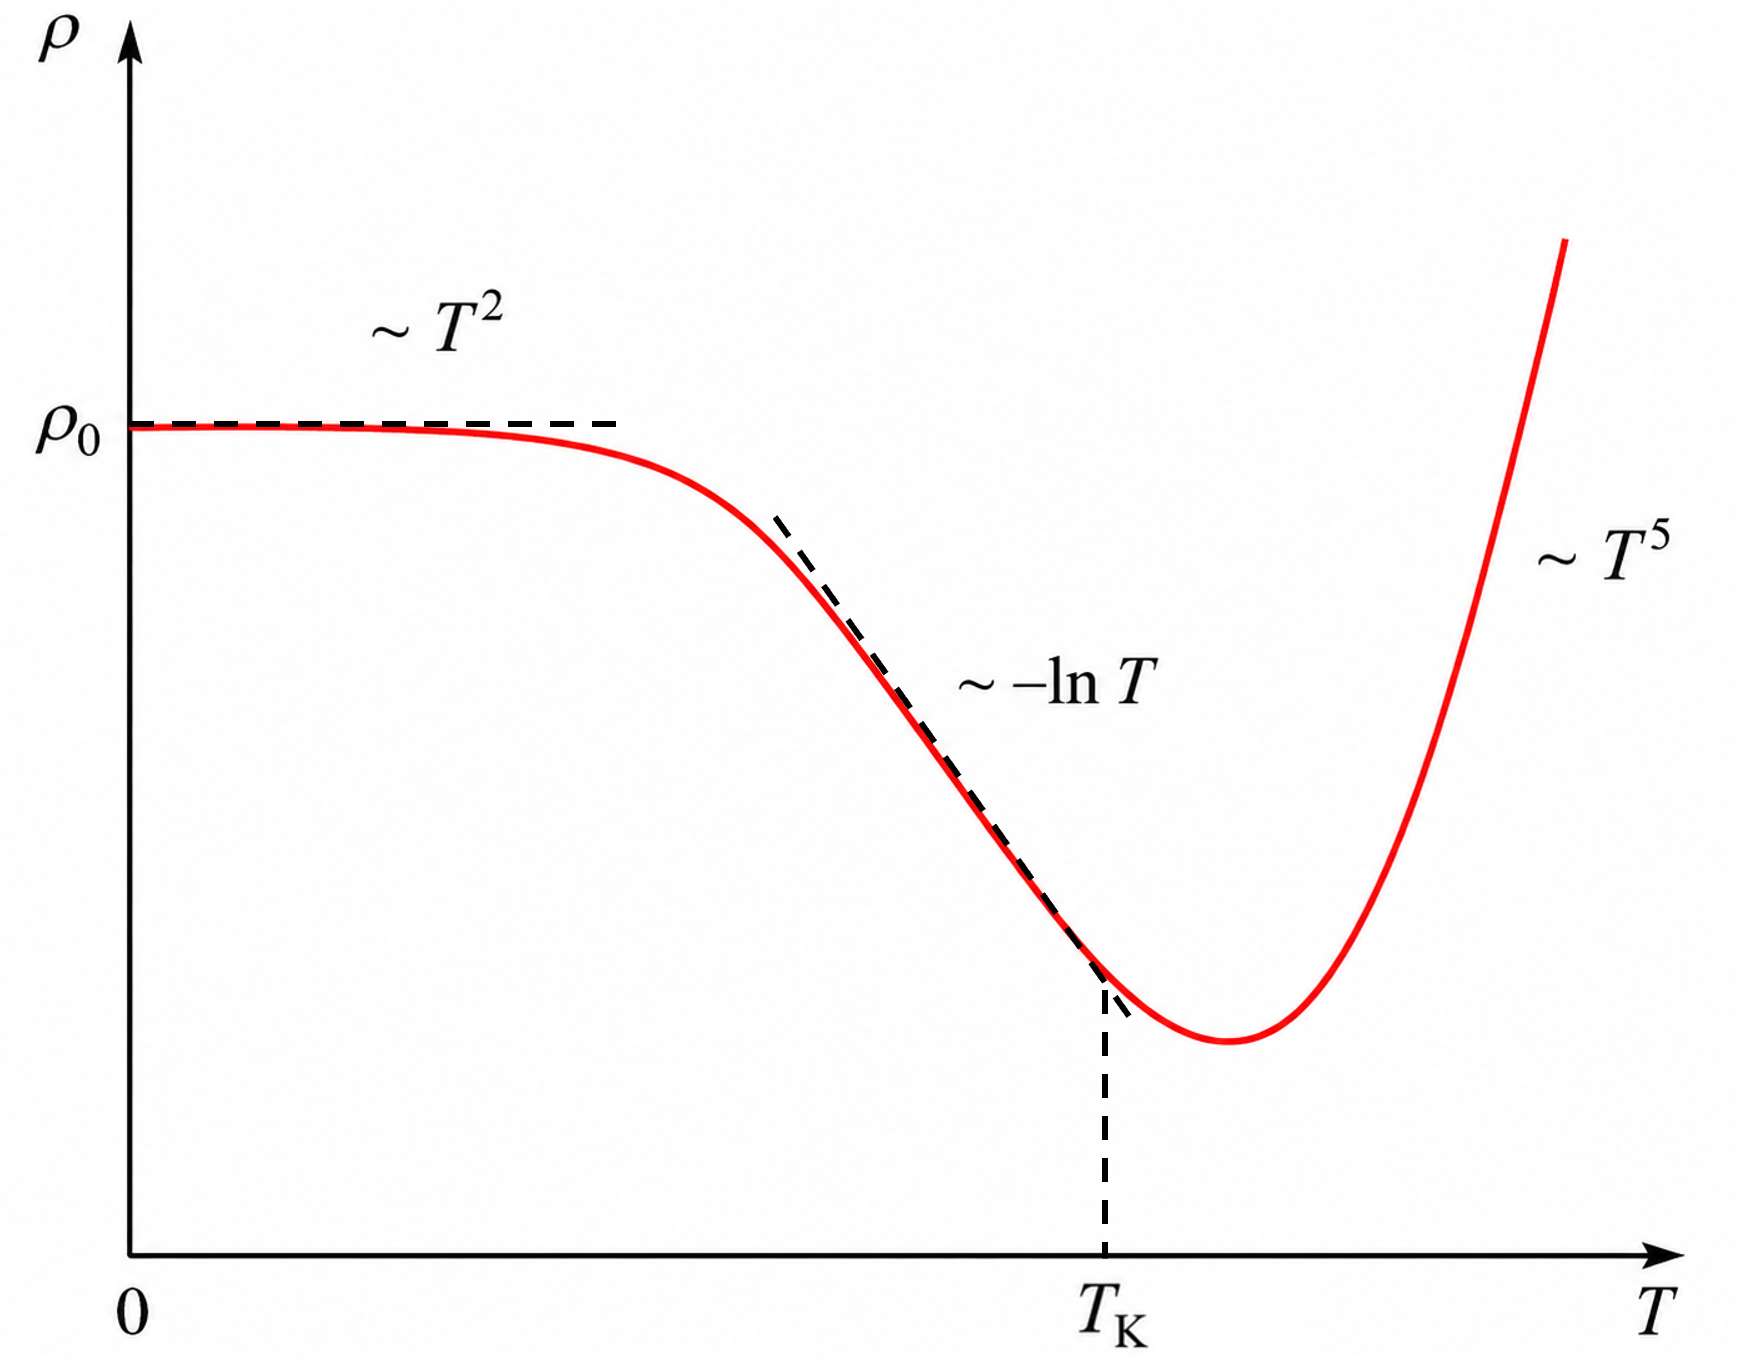
\includegraphics[width=0.55\linewidth]{Kondo1.png}
    \caption{Kondo效应$\rho-T$示意图}
    \label{fig:kondo_rho}
\end{figure}

\section{Kondo效应理论模型}

\subsection{Anderson杂质模型}

Kondo效应最初由Anderson杂质模型描述，该模型考虑局域电子态与导电电子之间的杂化：

\begin{equation}
H=
\sum_{k\sigma}\epsilon_k c_{k\sigma}^{\dagger}c_{k\sigma}
+\epsilon_d\sum_{\sigma}n_{d\sigma}
+Un_{d\uparrow}n_{d\downarrow}
+V\sum_{k\sigma}
(c_{k\sigma}^{\dagger}d_{\sigma}+h.c.)
\end{equation}

其中，第一项表示导电电子能带，第二项表示局域电子轨道，$U$表示局域电子库仑相互作用，$V$表示局域态与导电电子之间的杂化强度。

当局域电子满足强关联条件：

\begin{equation}
U\gg V
\end{equation}

时，局域轨道形成稳定磁矩。


\subsection{Kondo交换模型}

在强关联极限下，Anderson模型可转化为Kondo交换模型：

\begin{equation}
H_K=J\bm{S}\cdot\bm{s}(0)
\end{equation}

其中$\bm{S}$表示局域磁矩，$\bm{s}(0)$表示杂质位置处导电电子自旋密度，$J$表示交换耦合常数。

当：

\begin{equation}
J>0
\end{equation}

即反铁磁交换作用时，导电电子通过自旋补偿局域磁矩，形成总自旋为零的Kondo单态。


\subsection{Kondo温度}

Kondo关联出现的特征温度定义为Kondo温度：

\begin{equation}
T_K=
D\exp
\left[
-\frac{1}{J\rho(E_F)}
\right]
\end{equation}

其中$D$为电子能带宽度，$\rho(E_F)$为费米能级态密度。

由于$T_K$对交换耦合呈指数依赖，因此电子结构的微小变化可能导致明显的Kondo温度变化。当：

\begin{equation}
T<T_K
\end{equation}

时，Kondo屏蔽效应占据主导。


\section{Kondo效应的低温输运特征}

\subsection{电阻-温度关系}

Kondo效应最典型的实验表现是低温电阻反常上升：

\begin{equation}
\rho(T)\propto-\ln T
\end{equation}

实验中通常存在电阻最低点：

\begin{equation}
\frac{d\rho}{dT}=0
\end{equation}

对应温度记为$T_{\min}$。

当温度低于$T_{\min}$后，Kondo自旋散射逐渐增强，使电阻重新升高。


\subsection{低温电阻饱和}

简单Kondo理论中的$-\ln T$行为在极低温不会无限增加。当：

\begin{equation}
T\ll T_K
\end{equation}

体系进入强耦合费米液体状态，电阻趋于饱和：

\begin{equation}
\rho(T)=\rho(0)+AT^2
\end{equation}

该行为反映Kondo屏蔽后的低能准粒子散射。


\subsection{磁阻特征}

外加磁场产生Zeeman能量：

\begin{equation}
E_Z=g\mu_BB
\end{equation}

其中$g$为朗德因子，$\mu_B$为玻尔磁子。

磁场削弱Kondo单态，使自旋翻转散射降低，因此产生负磁阻：

\begin{equation}
MR=
\frac{\rho(B)-\rho(0)}
{\rho(0)}
<0
\end{equation}

负磁阻是判断Kondo散射的重要辅助证据。


\subsection{Hall输运特征}

Hall系数定义为：

\begin{equation}
R_H=\frac{1}{ne}
\end{equation}

其中$n$为载流子浓度。

在含磁矩体系中，Hall电阻可表示为：

\begin{equation}
R_{xy}=R_0B+R_sM
\end{equation}

其中第一项为普通Hall贡献，第二项为异常Hall贡献。

Kondo关联可能通过自旋相关散射和电子结构重整化导致Hall响应异常。


\section{镍酸盐体系中的Kondo-like行为}

\subsection{NdNiO$_3$中的局域磁矩}

稀土镍酸盐$RNiO_3$（例如NdNiO$_3$）属于典型强关联氧化物体系。

其电子结构具有明显的Ni-$3d$/O-$2p$杂化特征，可描述为：

\begin{equation}
Ni^{3+}\rightarrow Ni^{2+}+\underline{L}
\end{equation}

其中$\underline{L}$表示氧配体空穴。

由于Ni $3d$电子局域化，氧空位、外延应变以及界面电荷转移等因素可能产生局域磁矩：

\begin{equation}
S=\frac{1}{2},1
\end{equation}

这些局域磁矩可以与导电载流子发生交换耦合：

\begin{equation}
H_K=J\bm{S}_{Ni}\cdot\bm{s}
\end{equation}


\subsection{低温输运判据}

NdNiO$_3$薄膜中的低温电阻上升可能来源于多种机制，包括：

\begin{itemize}
\item Kondo自旋散射；
\item 弱局域化(weak localization)；
\item 电子-电子相互作用；
\item 变程跳跃输运。
\end{itemize}

因此，需要综合分析：

\begin{equation}
\rho(T),\quad MR(B,T),\quad R_H(T)
\end{equation}

其中：

\begin{itemize}
\item $\rho(T)$用于判断$-\ln T$行为；
\item $MR(B)$用于判断磁场对自旋散射的影响；
\item Hall输运用于分析载流子和异常散射机制。
\end{itemize}


\subsection{与其他低温机制区分}

弱局域化和电子-电子相互作用同样可能产生低温电阻增加，因此不能仅依据：

\begin{equation}
\rho(T)\sim-\ln T
\end{equation}

判断Kondo效应。

对于绝缘态镍酸盐，还需要考虑变程跳跃模型：

\begin{equation}
\rho(T)=
\rho_0
\exp
\left[
\left(
\frac{T_0}{T}
\right)^p
\right]
\end{equation}

因此，需要结合拟合温区、磁阻行为以及材料结构信息进行综合判断。


\section{总结}

Kondo效应来源于局域磁矩与导电电子之间的反铁磁交换耦合，其核心过程为：

\begin{equation}
\text{局域磁矩}
+
\text{导电电子}
\rightarrow
\text{Kondo单态}
\end{equation}

其主要输运特征包括：

\begin{itemize}
\item 低温电阻满足$\rho(T)\sim-\ln T$；
\item 存在电阻最低点$T_{\min}$；
\item 极低温出现电阻饱和；
\item 外磁场导致负磁阻；
\item Hall输运可能出现异常响应。
\end{itemize}

对于NdNiO$_3$等镍酸盐体系，Kondo-like行为体现了Ni $3d$局域电子与导电载流子之间的强关联耦合，是理解低温异常输运的重要机制之一。

\end{document}